\subsubsection{Photo-evaporation of a dense clump}
\label{sec.tests.raytracing}

The photo-evaporation of dense clumps of gas is prevalent in radiation
hydrodynamics simulations, and this test problem examines the
ionization front propagation into the dense clump, shadowing effects
behind the clump, and the hydrodynamic response on the clump from
photo-heating, all using \enzo's Moray ray-tracing module.  The
problem setup is the same as Test 7 in the Cosmological Radiative
Transfer Comparison Project \citep{IlievEtAl2009} and
\citet{Wise11_Moray}.  The simulation domain is 6.6~kpc on a side with
an ambient medium of pure neutral hydrogen $n_{\rm H} = 2 \times
10^{-4}\; \cubecm$ and $T = 8000 \unit{K}$.  We place a spherical
overdensity in hydrostatic equilibrium with the ambient medium.  It
has a radius $r = 0.8 \unit{kpc}$, hydrogen density $n_{\rm H} = 0.04
\cubecm$, and temperature $T = 40$ K, and it is centered at $(x,y,z) =
(5, 3.3, 3.3) \unit{kpc}$.  In \citet{IlievEtAl2009}, all of the codes
used a fixed $128^3$ grid to ease the comparison, but in this test to
demonstrate a higher resolution AMR solution, we employ a $128^3$ grid
with two additional levels of refinement with cells with a baryon mass
(method 2 in Section~\ref{sec:refinement_criteria}) greater than 1.5
being flagged for refinement.  This test is run for 15 Myr.

This cloud is subject to radiation from a point source at the center
of the $x=0$ boundary with an ionizing photon luminosity
$\dot{N}_\gamma = 3 \times 10^{51}$ photons s$^{-1}$, corresponding to
a flux $F_0 = 10^6 \unit{photons s}^{-1} \unit{cm}^{-2}$ at the clump
surface closest to the radiation source.  The radiation source has a
spectrum of a $T = 10^5 \unit{K}$ blackbody, and we use four energy
groups with the following mean energies and relative luminosities:
$E_i = (17.98, 31.15, 49.09, 76.98) \unit{eV}, L_i/L = (0.23, 0.36,
0.24, 0.06)$ that are optimized to reduce errors in the solutions with
a full spectrum and energy discretization \citep{Mirocha12}.
\citep[Note that this choice of energy groups is different
from][]{Wise11_Moray}.  We use a minimum angular resolution of 10 rays
per cell and a constant radiative transfer timestep of 25 kyr.  Figure
\ref{fig:shadowing} depicts the clump after at $t = 15$ Myr with the
outer layers expanding after being photo-heated.  It also shows the
sharp shadowing effects of the dense clump in the neutral fraction
plot that is representative of ray tracing techniques.

\begin{figure}
  \centering
  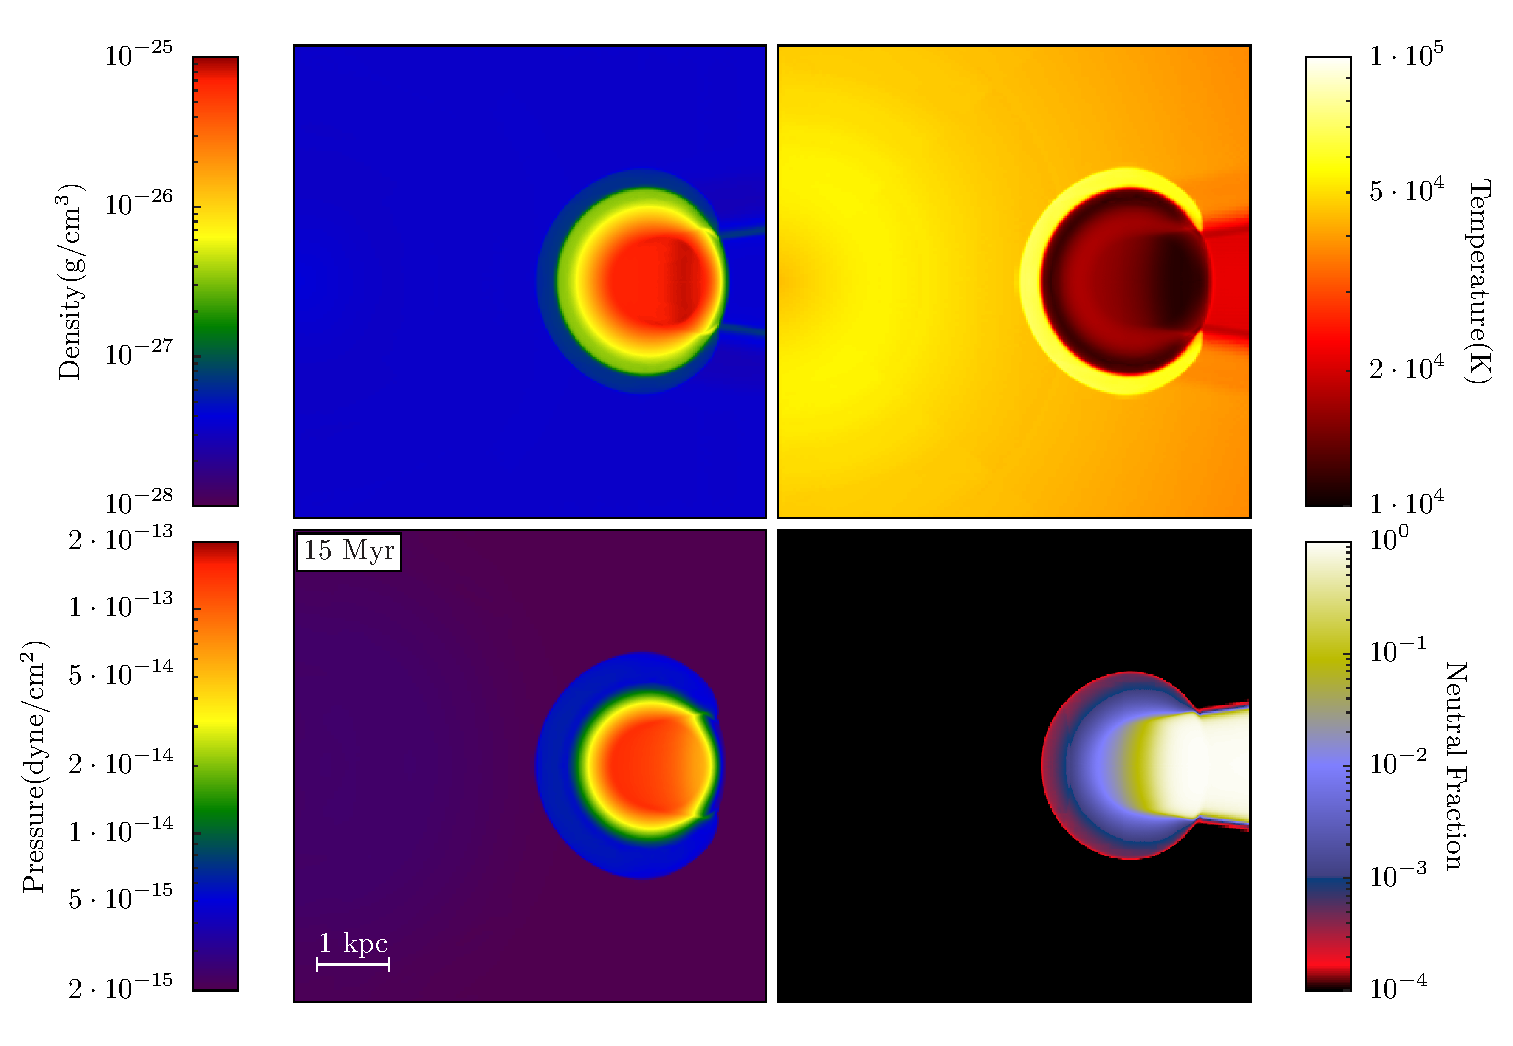
\includegraphics[width=1.0\textwidth]{figures/code-test-shadowing.eps}
  \caption{Photo-evaporation of a dense clump using the Moray
ray-tracing module.  Clockwise from the upper left corner: slices
through the clump center of the density, temperature, neutral hydrogen
fraction, and pressure at $t=15$~Myr after the initialization of the
simulation.  A point source of radiation is at the center of the -x
boundary and illuminates the clump with a constant luminosity, casting
a clear shadow behind the clump, as seen in the neutral hydrogen
fraction.}
  \label{fig:shadowing}
\end{figure}
